\documentclass[11pt, letterpaper]{article}

% Essential Packages
\usepackage[utf8]{inputenc}       % Encoding
\usepackage[T1]{fontenc}          % Font encoding
\usepackage[margin=1in]{geometry} % Page margins
\usepackage{graphicx}             % For inserting images
\usepackage{amsmath, amssymb}     % For math equations and symbols
\usepackage{hyperref}             % For clickable links and references
\usepackage{cite}                 % For handling numerical citations
\usepackage{indentfirst}
\usepackage{booktabs}
\usepackage{float}
% This layout/template was made from help with gemini AI. Quick google search of "Give me a template for latex journal article". Aside from that (the \usepackage layouts, the basic formating of major sections (not subsections)), everything was written by me.
% Doug said it was a-okay for using AI for this purpose ONLY. No writing or any text actually shown inside this document is from AI.


% Title Information
\title{Modeling Survival Risk in Oligodendroglioma: A Multi-Layer Molecular Prognostic Score}
\author{
    Oliver Strayer\\   
}
\date{July 2026} 

\begin{document}

\maketitle

\begin{abstract}
This paper analyzes the molecular features that drive the enormous range in oligodendroglioma survival, where patients live anywhere from under a year to over two decades despite sharing the same diagnosis. This study analyzes the molecular features driving this clinical mystery by constructing a multi-layered risk model. To ensure cohort purity, 187 histologically diagnosed patients from The Cancer Genome Atlas were molecularly screened; 32\% lacked definitive oligodendroglioma markers and were excluded, leaving 127 molecularly confirmed cases for analysis. A risk model was developed incorporating secondary oncogene mutations, PAX5 promoter methylation, and a 9-gene transcriptomic risk score through LASSO-penalized Cox regression. Secondary oncogene mutations independently doubled the risk of disease progression (HR = 2.55, p = 0.008). 

Combining these genetic, epigenetic, and transcriptomic features yielded a combined model with a concordance index of 0.84 (optimism-corrected bootstrap = 0.82). The transcriptomic score was successfully validated in an independent Chinese Glioma Genome Atlas cohort (n = 171, log-rank p = 0.030). Finally, the comprehensive model was translated into a clinically applicable two-variable nomogram. Limitations and ongoing validation within a third, international cohort are discussed.
\end{abstract}

\section{Introduction}
Oligodendroglioma is described as one of the more favorable diagnosis in the broader glioma family, but inside the oligodendroglioma family the survival rate varies enormously. Patients with the same diagnosis of IDH mutation and 1p/19q co-deletion (the standard for oligodendroglioma diagnosis \cite{WHO2021}) can live anywhere from under a year to past twenty \cite{CancerGenomeAtlas2015}. My father was diagnosed with this tumor as well, but standard markers couldn't answer how the tumor will affect his survival rate specifically. Standard markers simply were not enough. 

IDH mutation and 1p/19q co-deletion are the current markers that define oligodendroglioma \cite{WHO2021}. But, leaving the story at that leaves a huge amount of individual variation unaccounted for, and figuring out why some patients do so much better or worse than others within this same molecular category is the problem this project set out to address.

Other researchers have looked into details of this before. NOTCH1 mutations have been shown to predict worse outcomes in this exact molecular subtype \cite{Aoki2018}, and the PIK3 pathway, including PIK3CA has also been flagged as relevant \cite{CancerGenomeAtlas2015}. On the transcriptomic side, the POLA network published a LASSO-based risk score of eight-genes in oligodendroglioma using RNA-seq data \cite{Bertucci2023}. We will be using a LASSO-COX approach \cite{Friedman2010} (penalized regression to form a multi-gene risk score from RNA-seq data) \cite{Bertucci2023} for my own transcriptomic analysis \cite{Cox1972}.

On the epigenetic side, methylation markers are already an understood glioma prognosis. MGMT prognosis methylation, for example, is used to predict whether patients will respond to certain chemotherapy \cite{Hegi2005}. However, no methylation analysis has been done on my specific unique genes for oligodendroglioma. 

We will also be screening all datasets for molecularly confirmed oligodendroglioma, as in a lot of these datasets as mentioned earlier used a histological view of the tumor to classify it, resulting in a large discrepancy between actual oligodendroglioma and other gliomas. Although it makes the dataset slightly smaller, we did not want to accidentally put tumors of other classification into my model.

In total, this paper will be looking at RNA-sequence data, Methylation data, clinical variables, within a filtered cohort, validating said cohort on an independent cohort, and putting it all together in a multi-variable, layered risk model and nomogram.

\section{Methodology}

\subsection{Discovery Cohort and Molecular Filtering}

Clinical, histological, mutation, RNA-seq, and methylation data were obtained from The Cancer Genome Atlas Low-Grade Glioma project (TCGA-LGG, from the USCS-Xena Portal) \cite{Goldman2020}. The full TCGA-LGG dataset contains 530 patients, of which 198 had a histological diagnosis of oligodendroglioma, distinct from astrocytoma (n=197) and oligoastrocytoma (n=134). After removing patients with missing survival data, 197 histologically diagnosed oligodendroglioma patients remained.

Mutation status was obtained for eight genes commonly altered in low-grade glioma: IDH1, IDH2, TERT, CIC, FUBP1, ATRX, NOTCH1, and PIK3CA. In my process, these were referred to as "Major Biological Signatures" with RNA-sequence genes as "Minor Biological Signatures." Merging clinical and mutation data reduced the cohort to 187 patients with complete data across all eight genes.

However, histological diagnosis alone does not guarantee that a tumor meets the molecular definition of oligodendroglioma. Using the \texttt{IDH\_CODEL\_SUBTYPE} classification, this 187-patient cohort was found to include 127 patients molecularly confirmed as IDH-mutant, 1p/19q co-deleted (IDHmut-codel, the basis for oligodendroglioma \cite{WHO2021}), alongside 41 IDH-mutant, non-co-deleted patients and 19 IDH-wildtype patients, both of which are more consistent with astrocytoma than true oligodendroglioma under WHO classification. The 60 patients (32.1\% of 187) failing to meet strict molecular criteria were removed from the dataset, and all analyses contain only the 127 molecularly confirmed patients.

Tumor grade was encoded as a binary value (WHO Grade III = 1, Grade II = 0). Progression-free interval (PFI), rather than overall survival, was used as the primary outcome, expressed in years by dividing the reported time in days by 365.

\subsection{Secondary Oncogene Classification}

Mutations were labelled as oncogenic or tumor-suppressive using OncoKB \cite{OncoKB2017}. Within the molecularly confirmed cohort, this identified 37 patients with a secondary oncogenic mutation and 93 patients with a tumor-suppressor mutation (mean oncogenic score 0.339, mean tumor-suppressor score 0.953, reflecting the relative frequency of each mutation class). Because tumor-suppressor mutations were common and expected in this population (e.g., ATRX, FUBP1) and did not show independent prognostic value in preliminary testing, this analysis focuses specifically on secondary oncogene mutations, defined as the presence of NOTCH1 and/or PIK3CA, as these represent additional oncogenic events beyond the IDH1/1p19q-defining mutations. This was encoded as both a binary indicator (secondary oncogene present/absent) and a mutation  count (sum of NOTCH1 and PIK3CA mutations per patient, 0-2).

\subsection{Transcriptomic Risk Score}

RNA-seq expression data covering 20,530 genes were available for the 127 molecularly confirmed patients. Genes were filtered by mean-variance criteria to remove low-information transcripts, retaining 16,014 genes prior to further filtering. LASSO-penalized Cox regression (R, using glmnet), 10-fold cross-validation (random seed 42), $\lambda$ selected as lambda.min = 0.116 was used to select genes independently associated with progression-free survival from the filtered candidate set, identifying 11 non-zero genes (Figure~\ref{fig:lasso-full-path}). For the largest lambda values, meaning the strongest shrinkage early in the process, glmnet didn't fully converge. This didn't affect the lambda.min model actually used.

\begin{figure}[h!]
    \centering
    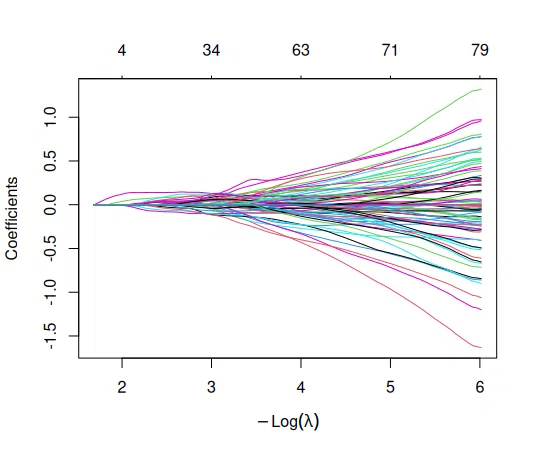
\includegraphics[width=0.75\linewidth]{Lasso_original.png}
    \caption{LASSO coefficient paths across all 16,014 candidate genes as function of regularization strength}
    \label{fig:lasso-full-path}
\end{figure}

The penalized Cox model was then re-fitted using only these 11 selected genes (coxph, survival package), which yielded the following coefficients used in all future and following analyzes: VEPH1 (0.190), ADAM6 (0.113), TRH (0.208), HLA-DQA2 (0.113), SIX1 (0.043), CENPV (--0.269), ABCC3 (0.253), DLX6 (0.222), C18orf34 (--0.272), PAX5 (0.370), and SEL1L3 (0.119). This refit model reached a concordance of 0.827 (n=125, 35 events) before incorporation into the larger multi-layer model. Figure~\ref{fig:lasso-selected-path} isolates the regularization paths of these 11 surviving genes from the full candidate set shown in Figure~\ref{fig:lasso-full-path}.

\begin{figure}[h!]
    \centering
    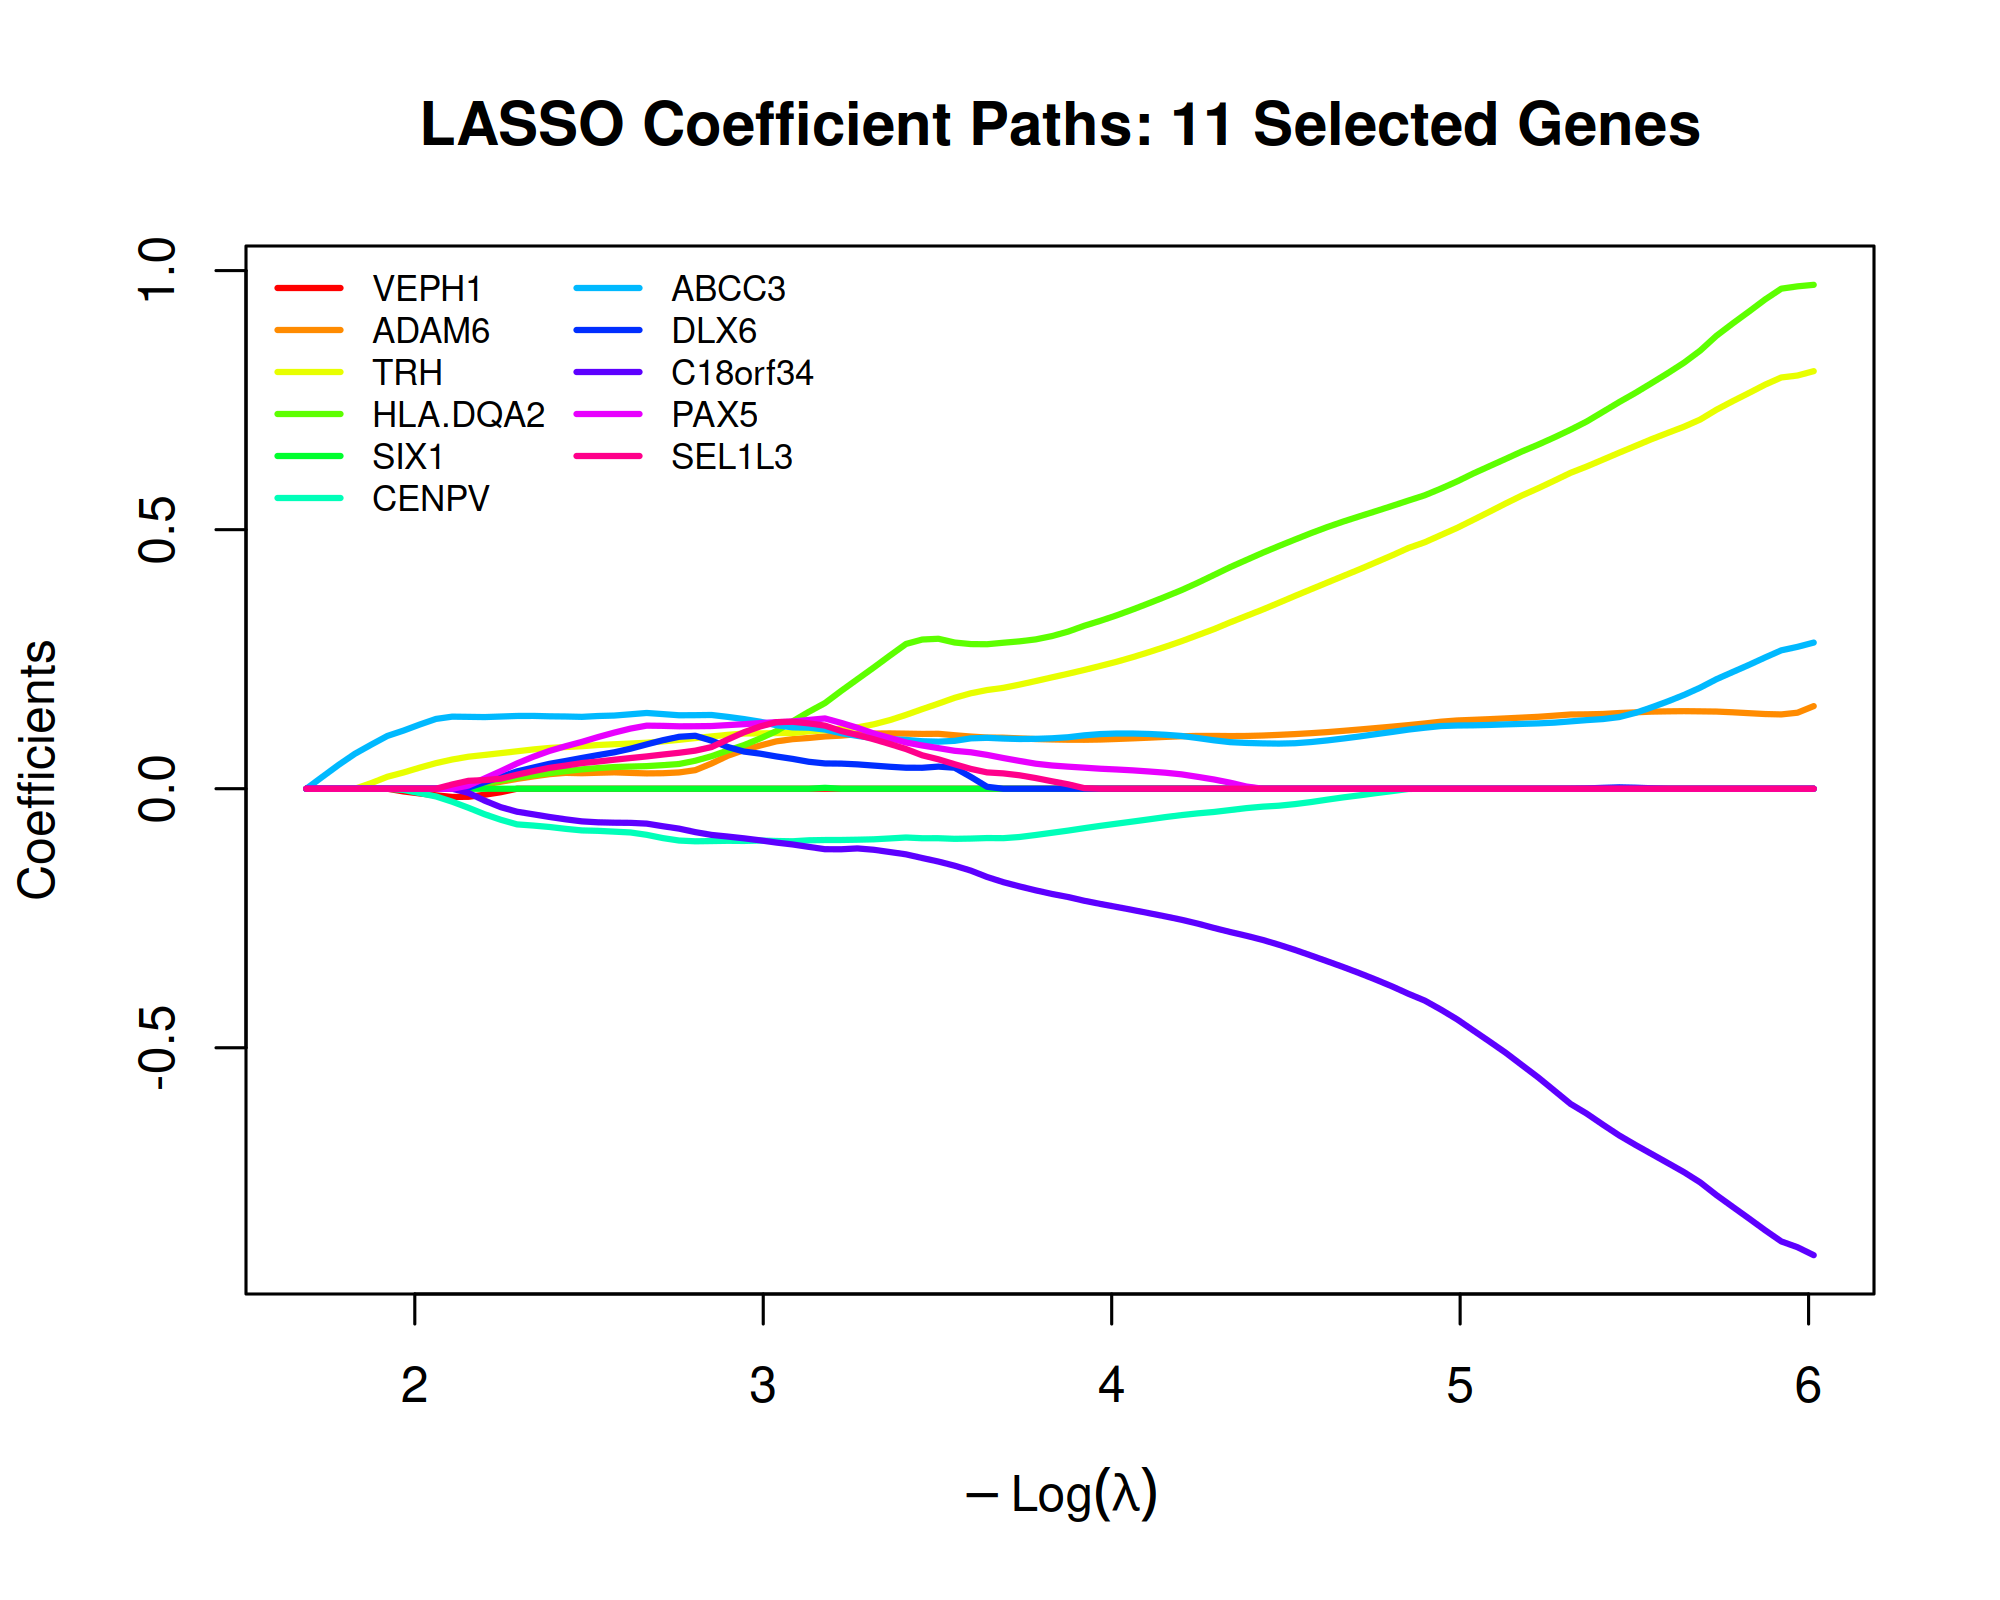
\includegraphics[width=0.75\linewidth]{17b_lasso_selected_genes.png}
    \caption{LASSO coefficient paths for the 11 genes selected at lambda.min from the full set in Figure~\ref{fig:lasso-full-path}.}
    \label{fig:lasso-selected-path}
\end{figure}

Unfortunately, two genes (ADAM6 and C18orf34) were dropped from the score as they were unavailable on the RNA-seq platform for external validation (CGGA cohort). These two genes may provide a more precise model once more datasets are available to validate them. The final 9-gene transcriptomic risk score for each patient was computed as the sum of each gene's expression value multiplied by its LASSO coefficient (beta).

\subsection{Gene Set Enrichment Analysis}

To assess whether the transcriptomic signature reflected coherent underlying biology rather than statistical artifact, genes were ranked by their association with high versus low-risk groups and tested for enrichment against the Hallmark, KEGG, and Reactome gene set collections using Gene Set Enrichment Analysis (GSEA) \cite{Subramanian2005}. All done through Python and gseapy. 


\subsection{Methylation Analysis}

Illumina HumanMethylation450 array data \cite{Bibikova2011} (485,577 probes across 530 patients) were filtered to probes located in gene promoter regions through a pre-defined promoter probe map. For PAX5, there were 5 specific probes. Other candidate genes, DLX6, SIX1, TRH, ABCC3, CENPV, MGMT, and CDKN2A, had probe counts ranging from 5 to 24 per gene. Methylation data was available for 127 patients, and 125 of them had complete clinical, mutation, and methylation data together. The other key minor biological signatures had no methylation data.

MGMT was included as a reference gene, or sanity check. Since its promoter methylation is an established, clinically validated prognostic marker in glioma \cite{Hegi2005}. Screening a well-characterized gene as well served as a check that the promoter-probe mapping pipeline was correctly identifying and using relevant probes before finding results about a gene with no prior literature in this disease. 

For all candidate minor biological signatures, promoter methylation beta-values across the 5 probes were averaged and multiplied by 100 to express methylation as a percentage. The relationship between PAX5 promoter methylation and PAX5 gene expression was found through Pearson correlation to understand the direction of the epigenetic-transcriptomic relationship before including methylation in the final survival model. This caution was to prevent accidental or meaningless correlation.

\subsection{Multi-Layer Cox Model}  

Cox proportional hazards models (Python, lifelines) were fit using progression-free interval as the outcome, with models built incrementally to assess the concordance contributed by each biological layer: (1) clinical variables only (age, grade); (2) clinical variables plus secondary oncogene status; (3) clinical variables, secondary oncogene status, and the transcriptomic risk score (penalizer = 0.1); and (4) a full model incorporating PAX5 promoter methylation (penalizer = 0.1) as well as all the layers prior. All models used the 125-patient cohort with complete data across all four layers to ensure concordance values were directly comparable across models.

\subsection{Bootstrap Optimism Correction}

Because concordance evaluated on the same data used to fit a model tends to be optimistic, Harrell's bootstrap optimism correction was applied to the full model. Five hundred bootstrap resamples were drawn with replacement (same size as the original 125-patient cohort, random seed 42). For each resample, a Cox model was refit and evaluated both on the resample itself and on the original cohort, with the difference between these two scores (the optimism) was averaged across all valid resamples and subtracted from the apparent concordance to yield a corrected estimate. Resamples with fewer than 5 observed events, or that failed to converge, were excluded from the average.

\subsection{External Validation}

The transcriptomic score was evaluated in a cohort of 171 molecularly confirmed oligodendroglioma patients from two Chinese Glioma Genome Atlas RNA-seq datasets (CGGA-325 and CGGA-693, merged together) \cite{Zhao2021}. Two genes in the original signature (ADAM6, C18orf34) were unavailable on the CGGA expression platform and were excluded from this analysis, leaving the same effective 9-gene score. Two distinct analyses were performed here and should be interpreted separately: first, the original TCGA-derived coefficients were applied without modification to CGGA patients to compute each patient's risk score, patients were split at the median score into high and low-risk groups, and survival curves were compared via log-rank test. This is a direct test of whether the original score generalizes to an independent population. Secondly, a separate Cox model was fit on CGGA data with each of the 9 genes as an independent covariate, allowing CGGA-specific coefficients to be found from scratch. The second model's concordance shows how informative these genes are within CGGA when refit, but not the portability of the original TCGA score. 

Clinical variables (grade, age) were separatedly validated on a distinct CGGA cohort of 182 molecularly confirmed oligodendroglioma patients, from the CGGA's broader dataset with 1018 total patients. Cox models were fit for these clinical variables individually within this cohort, and the results (p-values and hazard ratios) were compared against the clinical results from the TCGA discovery cohort as a cross-cohort consistency check. Chemotherapy and radiation was also looked at in this same cohort, but is not classified as validation due to TCGA not including either in its data.

As a further check on the major biological signatures, four of the eight genes used to define the discovery cohort's molecular signatures (NOTCH1, PIK3CA, CIC, FUBP1) were tested univariably as covariates in a Cox model on the same 182-patient CGGA clinical cohort. IDH1, IDH2, TERT, and ATRX were not tested here since IDH status was already used to filter the cohort to oligodendroglioma-specific patients only. In other words, it would not vary in the analysis as all 182 patients have IDH1/2 mutations.

\subsection{Nomogram Construction}

The full five-variable model (age, grade, secondary oncogene status, transcriptomic risk score, and PAX5 methylation) was simplified to two variables, secondary oncogene status and the transcriptomic risk score, for the nomogram. Age and grade were excluded due to their relatively small coefficient-weighted contribution to the full mode (section 3.6), and PAX5 methylation was excluded because its association with survival was significantly less once the transcriptomic risk score was introduced to the model (section 3.5), indicating overlapping rather than independent information. This simplification creates a nomogram that is visually usable and easily interpretable, at the cost of no longer reflecting every variable in the fully adjusted model. Due to this, it should be read as a simplified version of the full-risk tool/model rather than a portrayal of it in its entirety. 

\subsection{Patient-Level Prediction Tool}

In addition to the simplified nomogram, a patient-level prediction tool was built using the full five-variable model, accepting individual patient covariates (age, grade, secondary oncogene status, and gene expression values for the 9-gene signature) and outputting a predicted survival function, percentile rank against the training cohort, and risk classification. Two of these tools were created, one requiring input of a calculated gene score using the 9-gene signature among age, grade, and other variables, while the other just requires the input of a data file matching the structure of the TCGA RNA-seq dataset, automatically calculating the 9-gene signature risk score (still requiring input of the other variables, of course).

\subsection{Statistical Analysis}

All statistical analyses were performed in Python (lifelines, scikit-learn, gseapy) and R (glmnet, survival), with a two-sided significance threshold of $\alpha = 0.05$ throughout (bottom 5\% and top 5\%). Hazard ratios and confidence intervals from Cox models reflect Wald-based estimates as implemented in lifelines.

\section{Results}

\subsection{Cohort Characteristics and Molecular Misclassification}

Of the 187 histologically diagnosed oligodendroglioma patients with complete mutation data, 127 (67.9\%) were molecularly confirmed as IDH-mutant, 1p/19q co-deleted oligodendroglioma; the remaining 60 (32.1\%) did not meet molecular criteria despite their histological diagnosis, most commonly presenting as IDH-mutant without co-deletion or IDH-wildtype. All future results are restricted to the 127 molecularly confirmed patients.

\subsection{Secondary Oncogene Mutations}

In individual variable analysis, presence of a secondary oncogene mutation (NOTCH1 and/or PIK3CA) was associated with substantially worse progression-free survival (HR = 2.55, 95\% CI 1.27--5.13, p = 0.008). Median progression-free survival was 3.76 years among patients with a secondary oncogene mutation, compared to 8.11 years among those without (log-rank p = 0.006). This association remained significant in a model adjusted for age, grade, and PAX5 methylation (HR = 2.18, p = 0.037), but was attenuated and was less statistically significant once the transcriptomic risk score was added to the model (HR = 1.60, p = 0.143), suggesting overlap between the prognostic impact captured by secondary oncogene status and the transcriptomic score.

\begin{figure}[h]
    \centering
    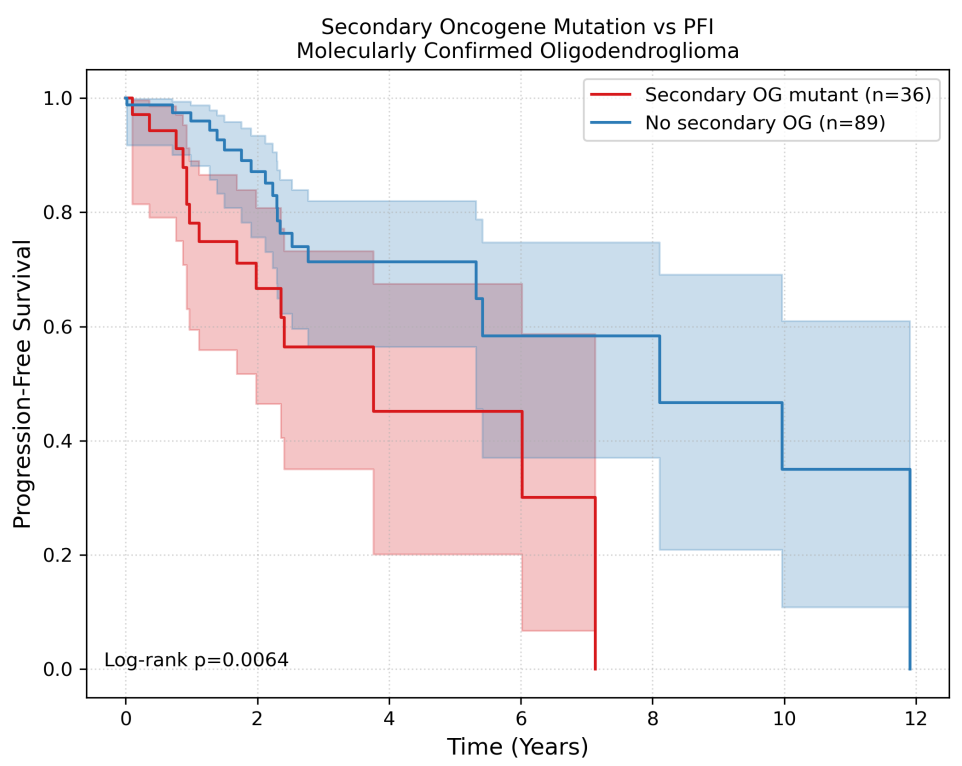
\includegraphics[width=0.75\linewidth]{Screenshot from 2026-07-27 15-06-45.png}
    \caption{Progression-free survival stratified by secondary oncogene mutation status (NOTCH1 and/or PIK3CA) in the molecularly confirmed TCGA discovery cohort (n=127).}
    \label{fig:secondary-og-km}
\end{figure}

\subsection{Transcriptomic Risk Score}

The 9-gene transcriptomic risk score, found as a linear combination of gene expression values weighted by their LASSO coefficients (Section~2.3), was independently prognostic inside the full five-variable model. After accounting for age, grade, secondary oncogene status, and PAX5 methylation simultaneously (HR = 1.81 per one-unit increase in score, p \textless 0.001), the 9-gene signature was still the most impactful. This was the highest hazard ratio of any single covariate in the full model. As detailed in Section~3.6, the transcriptomic score also contributed the highest increase in model concordance between the four biological layers tested. The biological coherence of the underlying gene signature is further examined through pathway enrichment analysis (Section~3.4, GSEA), and its generalization to an independent population is tested by external validation (Section~3.7).

\subsection{Gene Set Enrichment Analysis}

Ranking genes based on their association with the high versus low-risk groups defined by the transcriptomic score identified 7 significant Hallmark pathways, 2 significant KEGG pathways, and 25 significant Reactome pathways (Table~\ref{tab:gsea}, python gseapy) \cite{Hallmark2015}. The most strongly enriched pathways were filled with cell cycle and proliferation signatures, including the top two Hallmark pathways (G2-M Checkpoint, NES = 2.03; TNF-alpha Signaling via NF-kB, NES = 1.83) and the two most significant Reactome pathways (Cell Cycle, Mitotic, NES = 2.17; Cell Cycle, NES = 2.02). This pattern is consistent with known cancer proliferation biology, providing some biological plausibility and understanding for the transcriptomic score beyond its purely statistical derivation.

\begin{table}[h!]
\centering
\caption{Top enriched pathways by gene set collection}
\label{tab:gsea}
\begin{tabular}{llccc}
\toprule
Collection & Pathway & NES & Nominal $p$ & FDR $q$ \\
\midrule
Hallmark & G2-M Checkpoint & 2.03 & \textless 0.001 & \textless 0.001 \\
Hallmark & TNF-alpha Signaling via NF-kB & 1.83 & 0.002 & 0.010 \\
Hallmark & Inflammatory Response & 1.77 & 0.006 & 0.018 \\
Reactome & Cell Cycle, Mitotic & 2.17 & \textless 0.001 & \textless 0.001 \\
Reactome & Cell Cycle & 2.02 & \textless 0.001 & 0.003 \\
KEGG & Human T-cell Leukemia Virus 1 Infection & 2.09 & \textless 0.001 & 0.003 \\
\bottomrule
\end{tabular}
\end{table}

\begin{figure}[h!]
    \centering
    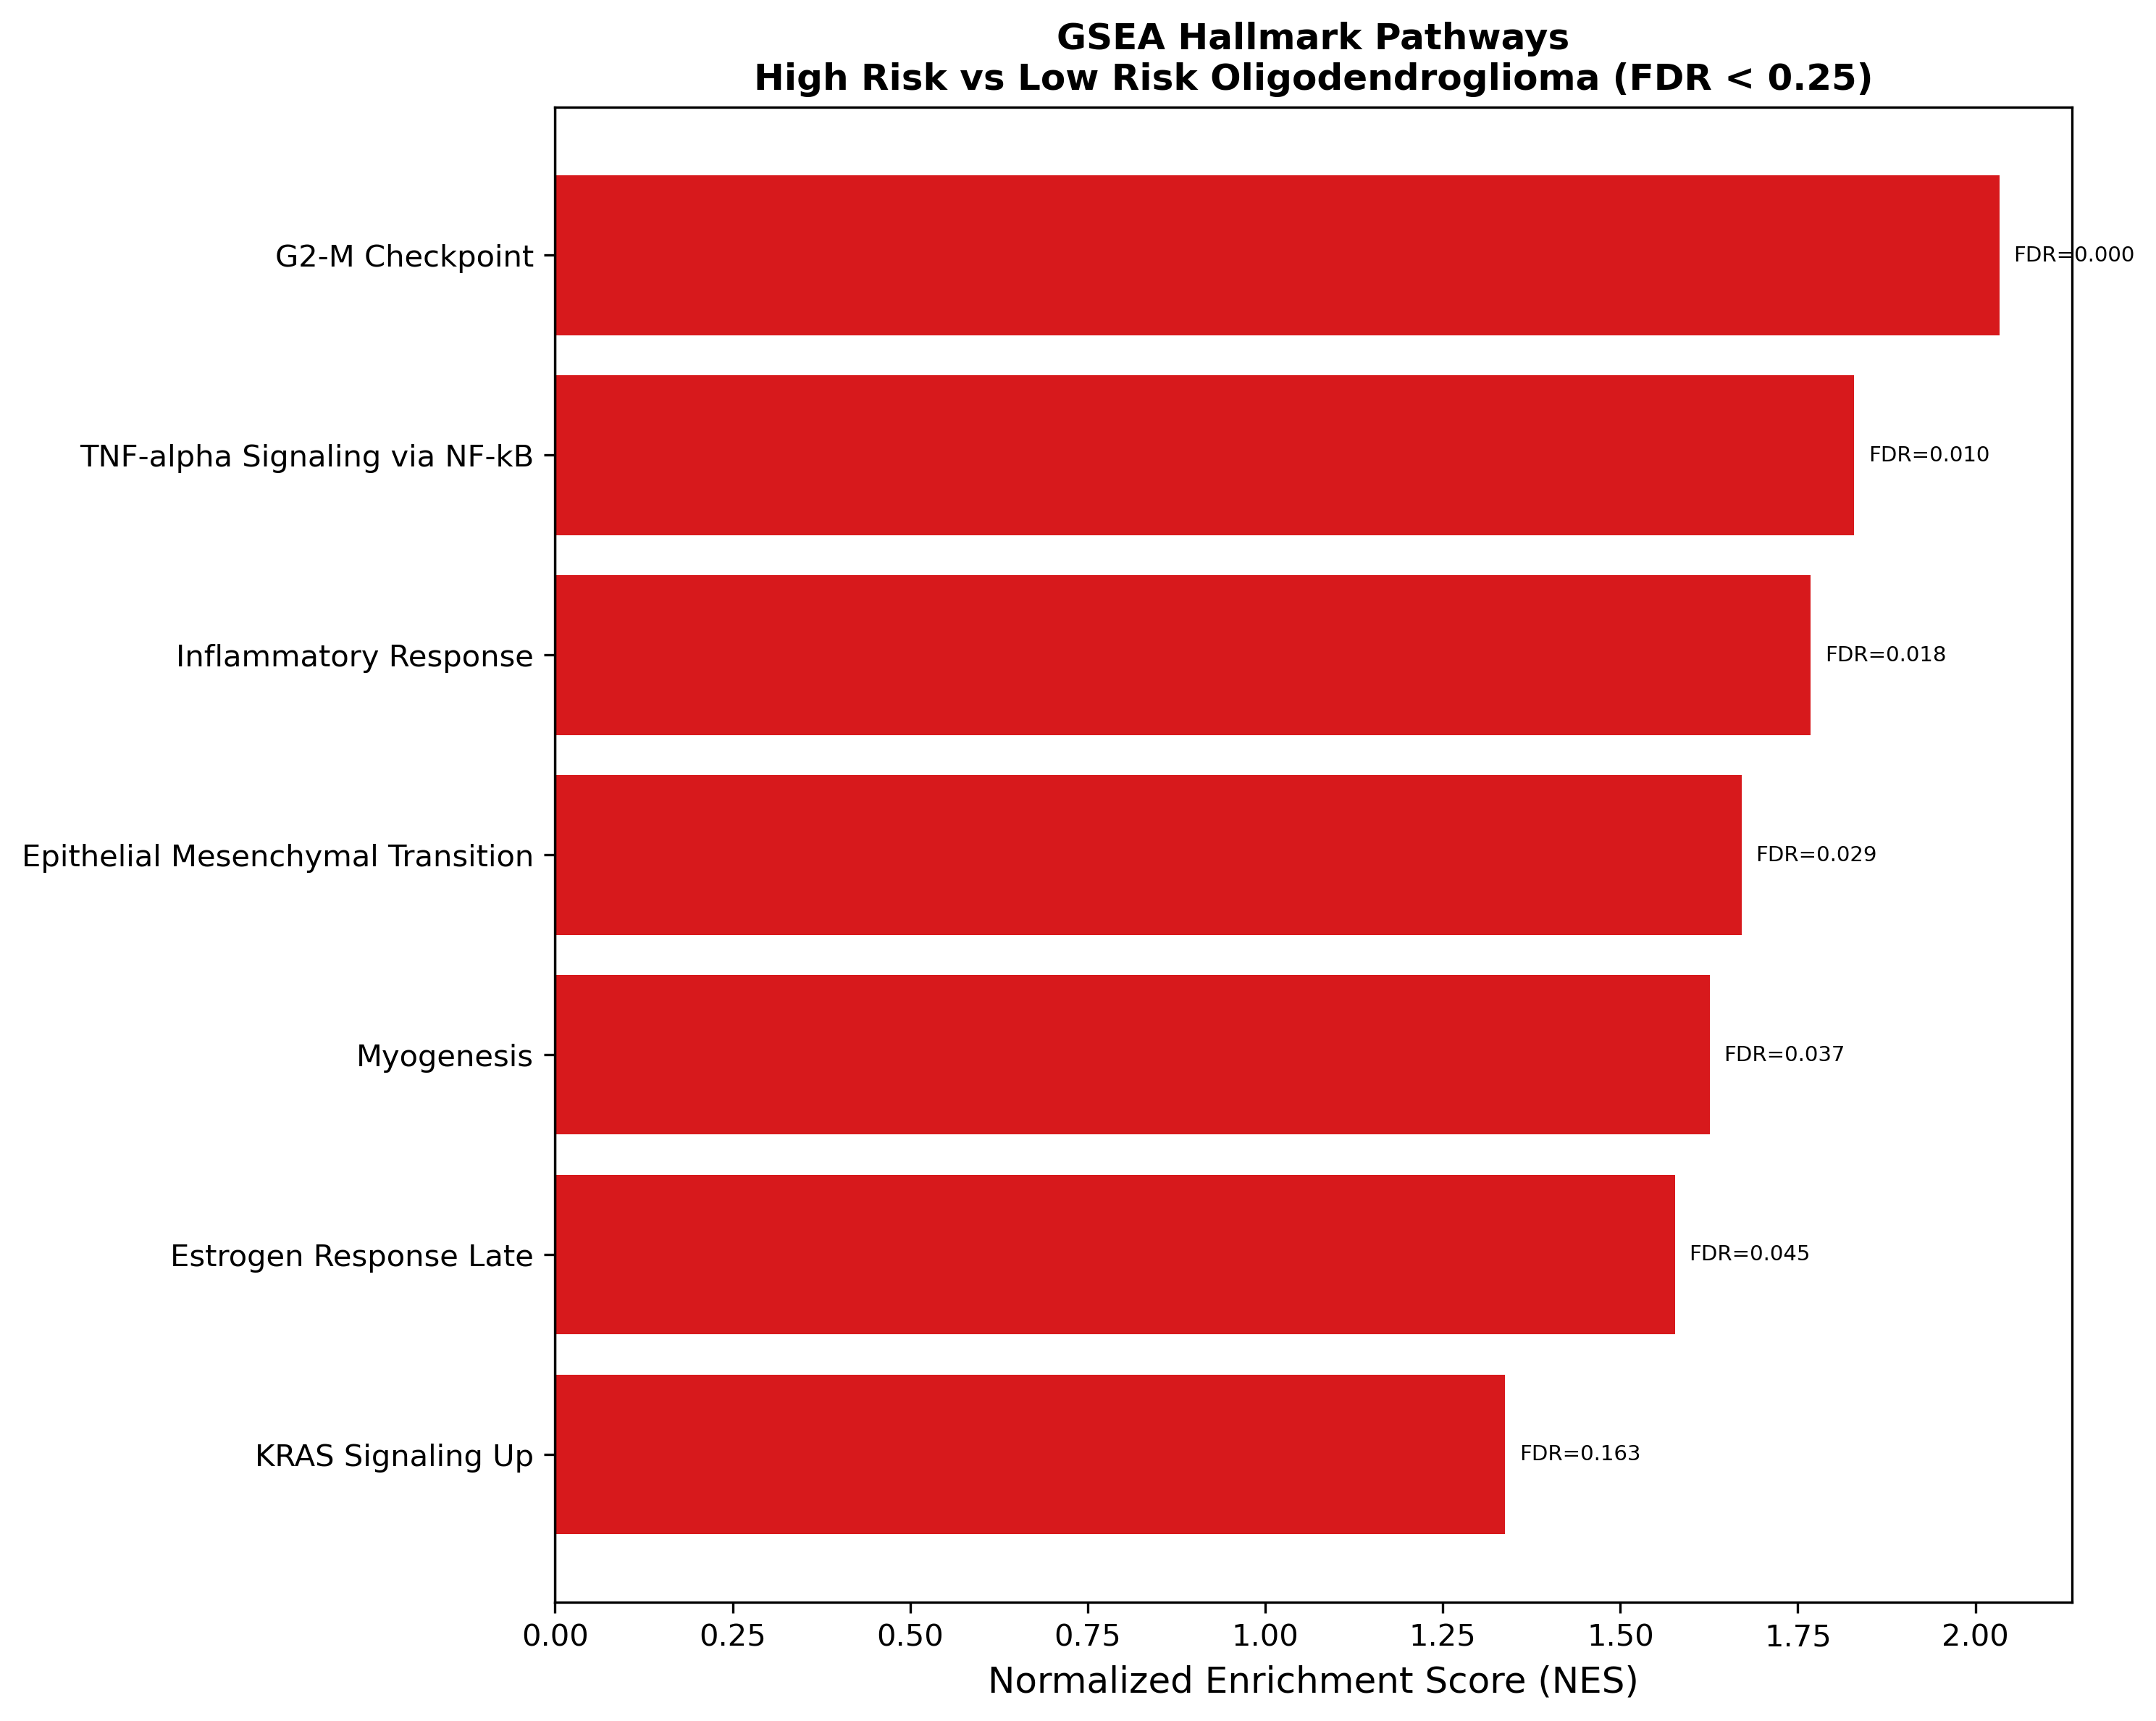
\includegraphics[width=0.75\linewidth]{06_gsea_hallmark.png}
    \caption{GSEA Reactome Pathway Enrichment Score}
    \label{fig:placeholder}
\end{figure}

\subsection{Methylation}

Across all eight candidate genes screened for promoter methylation (n=125), PAX5 showed the strongest univariate correlation with progression-free survival (HR = 1.060, p = 0.001), followed by CENPV, which approached but did not reach significance (HR = 1.041, p = 0.058 > 0.025). No other candidate gene, including MGMT, the reference gene included as a pipeline sanity check, reached significance in this screen (MGMT: HR = 1.007, p = 0.773; Table~\ref{tab:methylation-screen}). Given that MGMT promoter methylation is well established as clinically meaningful in glioma, its null result here most likely reflects that MGMT methylation is already common within this specific IDH-mutant, 1p/19q-codeleted subgroup. This leaves less variation for a survival model to search for within this narrower population, rather than a failure of the analysis pipeline itself.

\begin{table}[h!]
\centering
\caption{Univariate promoter methylation screen (n=125)}
\label{tab:methylation-screen}
\begin{tabular}{lcc}
\toprule
Gene & HR & $p$-value \\
\midrule
PAX5 & 1.060 & 0.001 \\
CENPV & 1.041 & 0.058 \\
TRH & 1.025 & 0.142 \\
SIX1 & 1.055 & 0.297 \\
ABCC3 & 1.016 & 0.340 \\
DLX6 & 1.018 & 0.452 \\
CDKN2A & 1.013 & 0.565 \\
MGMT & 1.007 & 0.773 \\
\bottomrule
\end{tabular}
\end{table}

PAX5 promoter methylation was positively correlated with PAX5 expression (r = 0.570, p < 0.001), a direction that goes against the typical expectation that promoter methylation silences transcription (discussed further in Section~4). In a model adjusted for age, grade, and secondary oncogene status, PAX5 methylation was an independent predictor of worse progression-free survival (HR = 1.042, 95\% CI 1.001--1.085, p = 0.046). This association was substantially reduced when the transcriptomic score was added to the same model (HR = 1.015, p = 0.344), suggesting overlapping between methylation and the transcriptomic layer rather than fully independent contributions.

\subsection{Multi-Layer Cox Model}

Concordance increased at each additional biological layer. Clinical variables alone reached 0.646, adding secondary oncogene status reached 0.707, and adding the transcriptomic score reached 0.841; the full model additionally incorporating PAX5 methylation also reached 0.841 (Table~\ref{tab:concordance}), indicating that methylation's contribution to ranking accuracy was already captured by the transcriptomic score once both were included together, consistent with the pattern observed in Sections~3.2 and 3.5.

Because apparent concordance evaluated on the same data used to fit a model tends to be optimistic and overfit, particularly given the sample size here (125 complete cases, 35 events, 5 covariates), bootstrap optimism correction was applied. This yielded a corrected concordance of 0.822 (mean optimism = 0.020 over 500 resamples; 95\% CI: 0.758--0.888).

\begin{table}[H]
\centering
\caption{Concordance by model layer}
\label{tab:concordance}
\begin{tabular}{lc}
\toprule
Model & Concordance \\
\midrule
Clinical only (age, grade) & 0.646 \\
Clinical + secondary oncogene & 0.707 \\
Clinical + secondary oncogene + transcriptomic score & 0.841 \\
Full model (+ PAX5 methylation) & 0.841 \\
Full model, bootstrap-corrected & 0.822 \\
\bottomrule
\end{tabular}
\end{table}

\begin{figure}[h!]
    \centering
    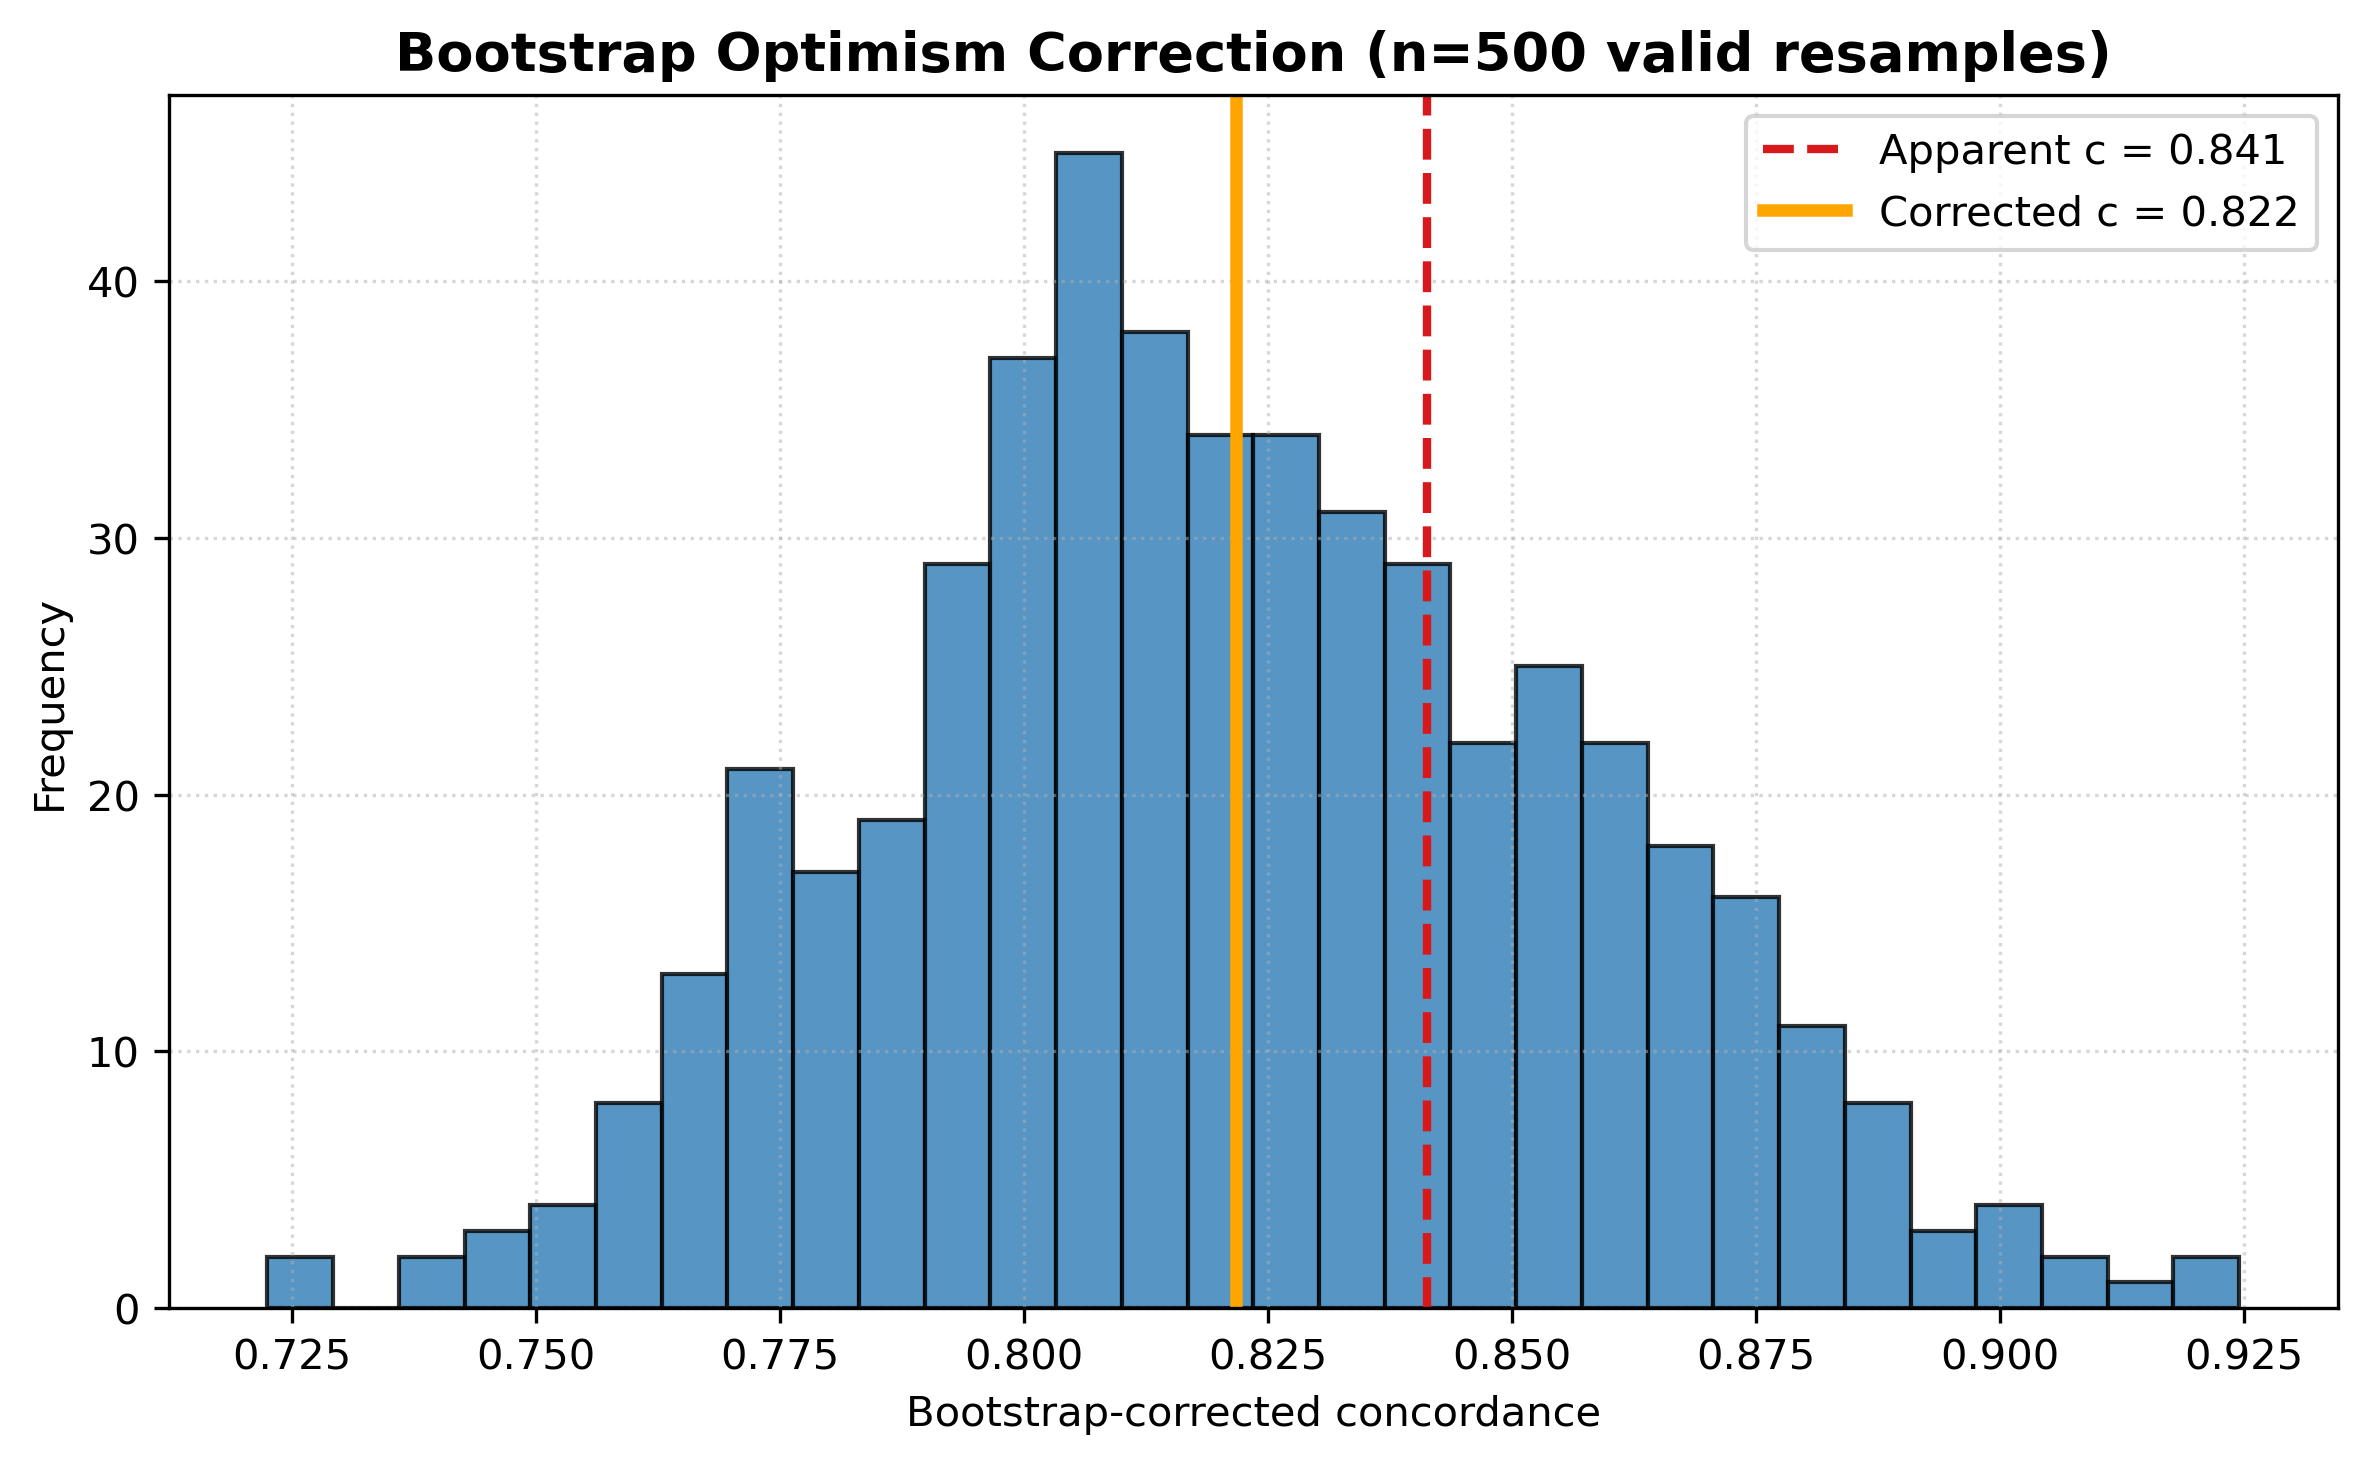
\includegraphics[width=0.75\linewidth]{14_bootstrap_correction.png}
    \caption{Bootstrap Optimism Concordance (n=500)}
    \label{fig:placeholder}
\end{figure}

\subsection{External Validation (CGGA)}

Applying the unmodified TCGA-derived transcriptomic score to an external cohort of 171 molecularly confirmed CGGA patients (Chinese Glioma Genome Atlas) produced significant separation between high and low-risk groups (log-rank p = 0.030), directly supporting the generalizability or the discovery cohort to an independent, internationally, ethnically distinct population. Refitting the 9-genomic covariate Cox model directly on CGGA data reached a concordance of 0.734, indicating these genes remain informative for survival when refit locally, though this result should not be interpreted as validating the original's concordance directly.

Clinical variables showed broadly consistent, though not uniformly significant, associations across the two independent cohorts (Table~\ref{tab:cgga-clinical}). In the CGGA clinical cohort, WHO Grade III was significantly associated with adverse survival (HR = 2.48, 95\% CI 1.38--4.46, p = 0.0025). This is consistent with grade's effect in TCGA, although grade failed to reach statistical significance. Age showed a similar association in both cohorts (CGGA: HR = 1.03, p = 0.052; TCGA: HR ranging from 1.02--1.03 across models, p = 0.03--0.29). 

\begin{table}[H]
\centering
\caption{Clinical variable comparison, TCGA discovery vs. CGGA validation cohort}
\label{tab:cgga-clinical}
\begin{tabular}{lcccc}
\toprule
Variable & TCGA HR (range) & TCGA $p$ (range) & CGGA HR & CGGA $p$ \\
\midrule
Grade (III vs. II) & 1.14--1.52 & 0.22--0.61 & 2.48 & 0.0025 \\
Age & 1.02--1.03 & 0.03--0.29 & 1.03 & 0.052 \\
\bottomrule
\end{tabular}
\end{table}

None of the four major biological signature genes tested individually (NOTCH1, PIK3CA, CIC, FUBP1) reached statistical significance in the CGGA clinical cohort (Table~\ref{tab:cgga-mutations}), with extremely wide confidence intervals in each case (e.g., PIK3CA: 95\% CI 0.54--43.33). This is consistent with the analysis being underpowered given the small number of mutation-positive patients within this cohort, rather than evidence against the prognostic relevance of these mutations established in this study and in prior literature.

\begin{table}[h!]
\centering
\caption{Major biological signature validation in CGGA clinical cohort (n=182)}
\label{tab:cgga-mutations}
\begin{tabular}{lccc}
\toprule
Gene & HR & 95\% CI & $p$-value \\
\midrule
PIK3CA & 4.82 & 0.54--43.33 & 0.161 \\
CIC & 0.39 & 0.07--2.08 & 0.272 \\
NOTCH1 & 0.45 & 0.05--3.77 & 0.464 \\
FUBP1 & 0.00 & 0.0--$\infty$ & 0.996 \\
\bottomrule
\end{tabular}
\end{table}

\begin{figure}[H]
    \centering
    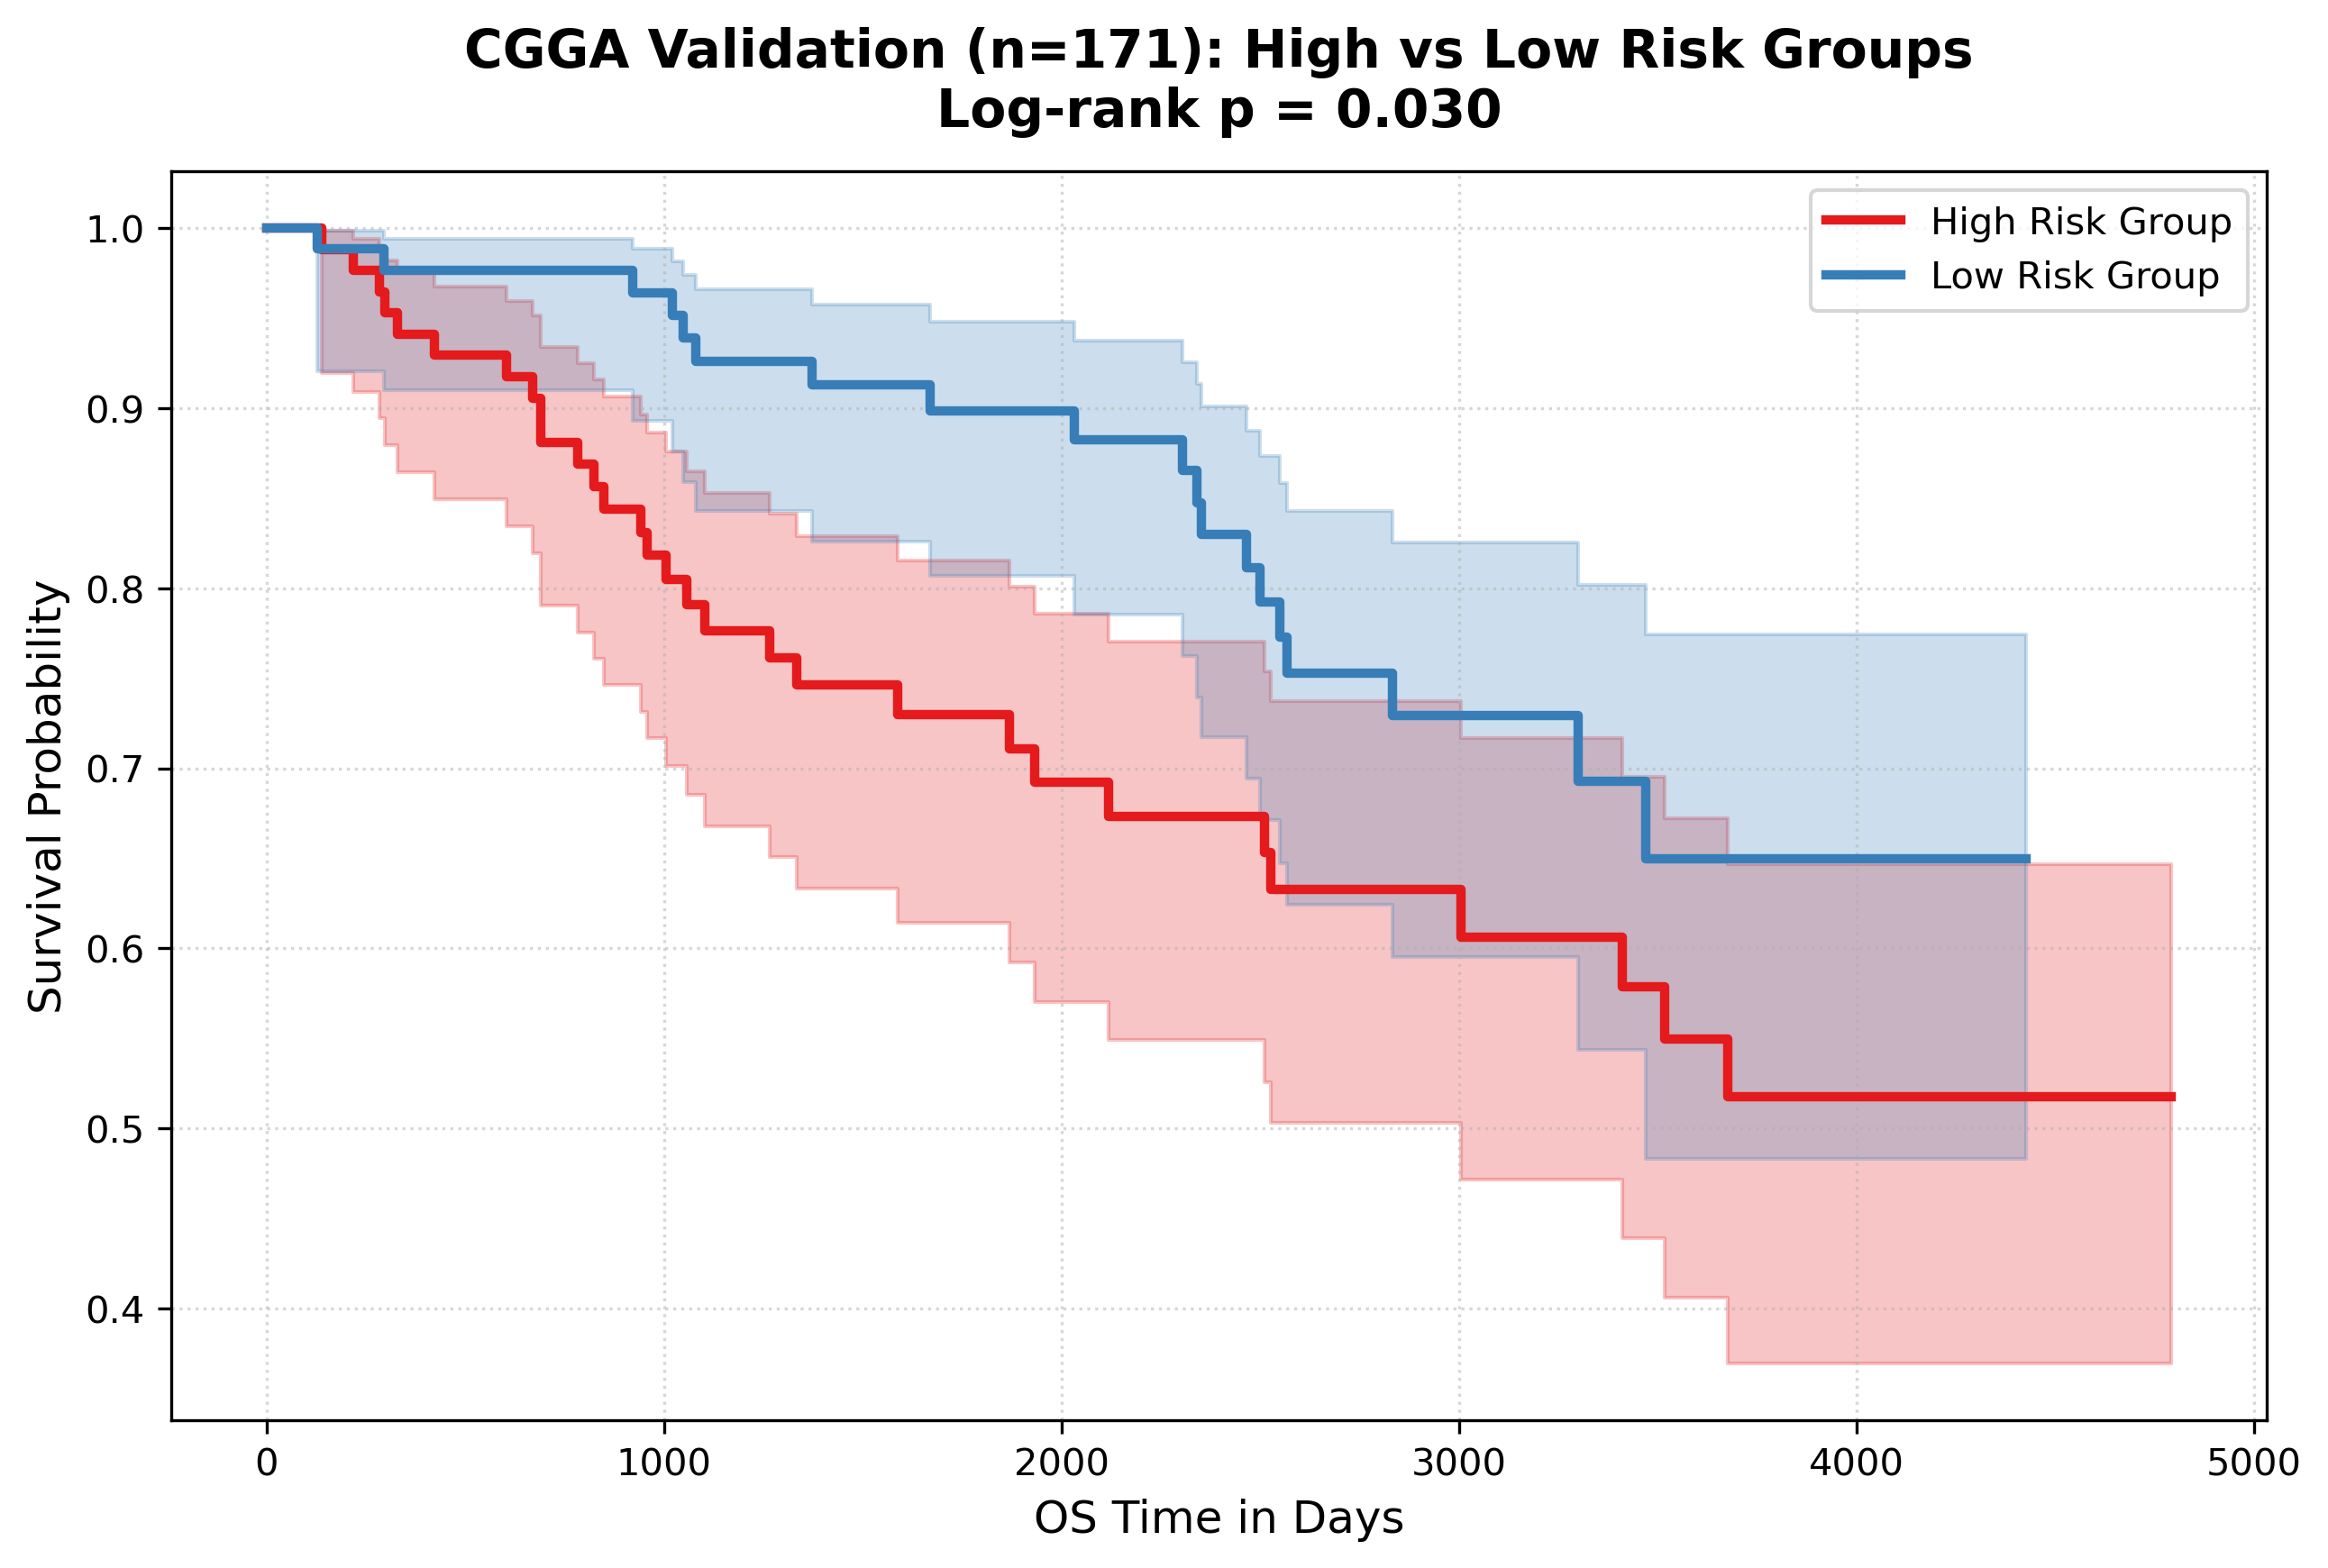
\includegraphics[width=0.75\linewidth]{KM_CCGA_validation.png}
    \caption{CGGA validation on purely the 9-gene transcriptomic score}
    \label{fig:placeholder}
\end{figure}

\subsection{Nomogram}

The full model was simplified into a two-variable nomogram (only secondary oncogene status and the transcriptomic score). The nomogram predicts progression-free survival probabilities at 3, 5, and 10 years (Figure~\ref{fig:nomogram}).

\begin{figure}[H]
    \centering
    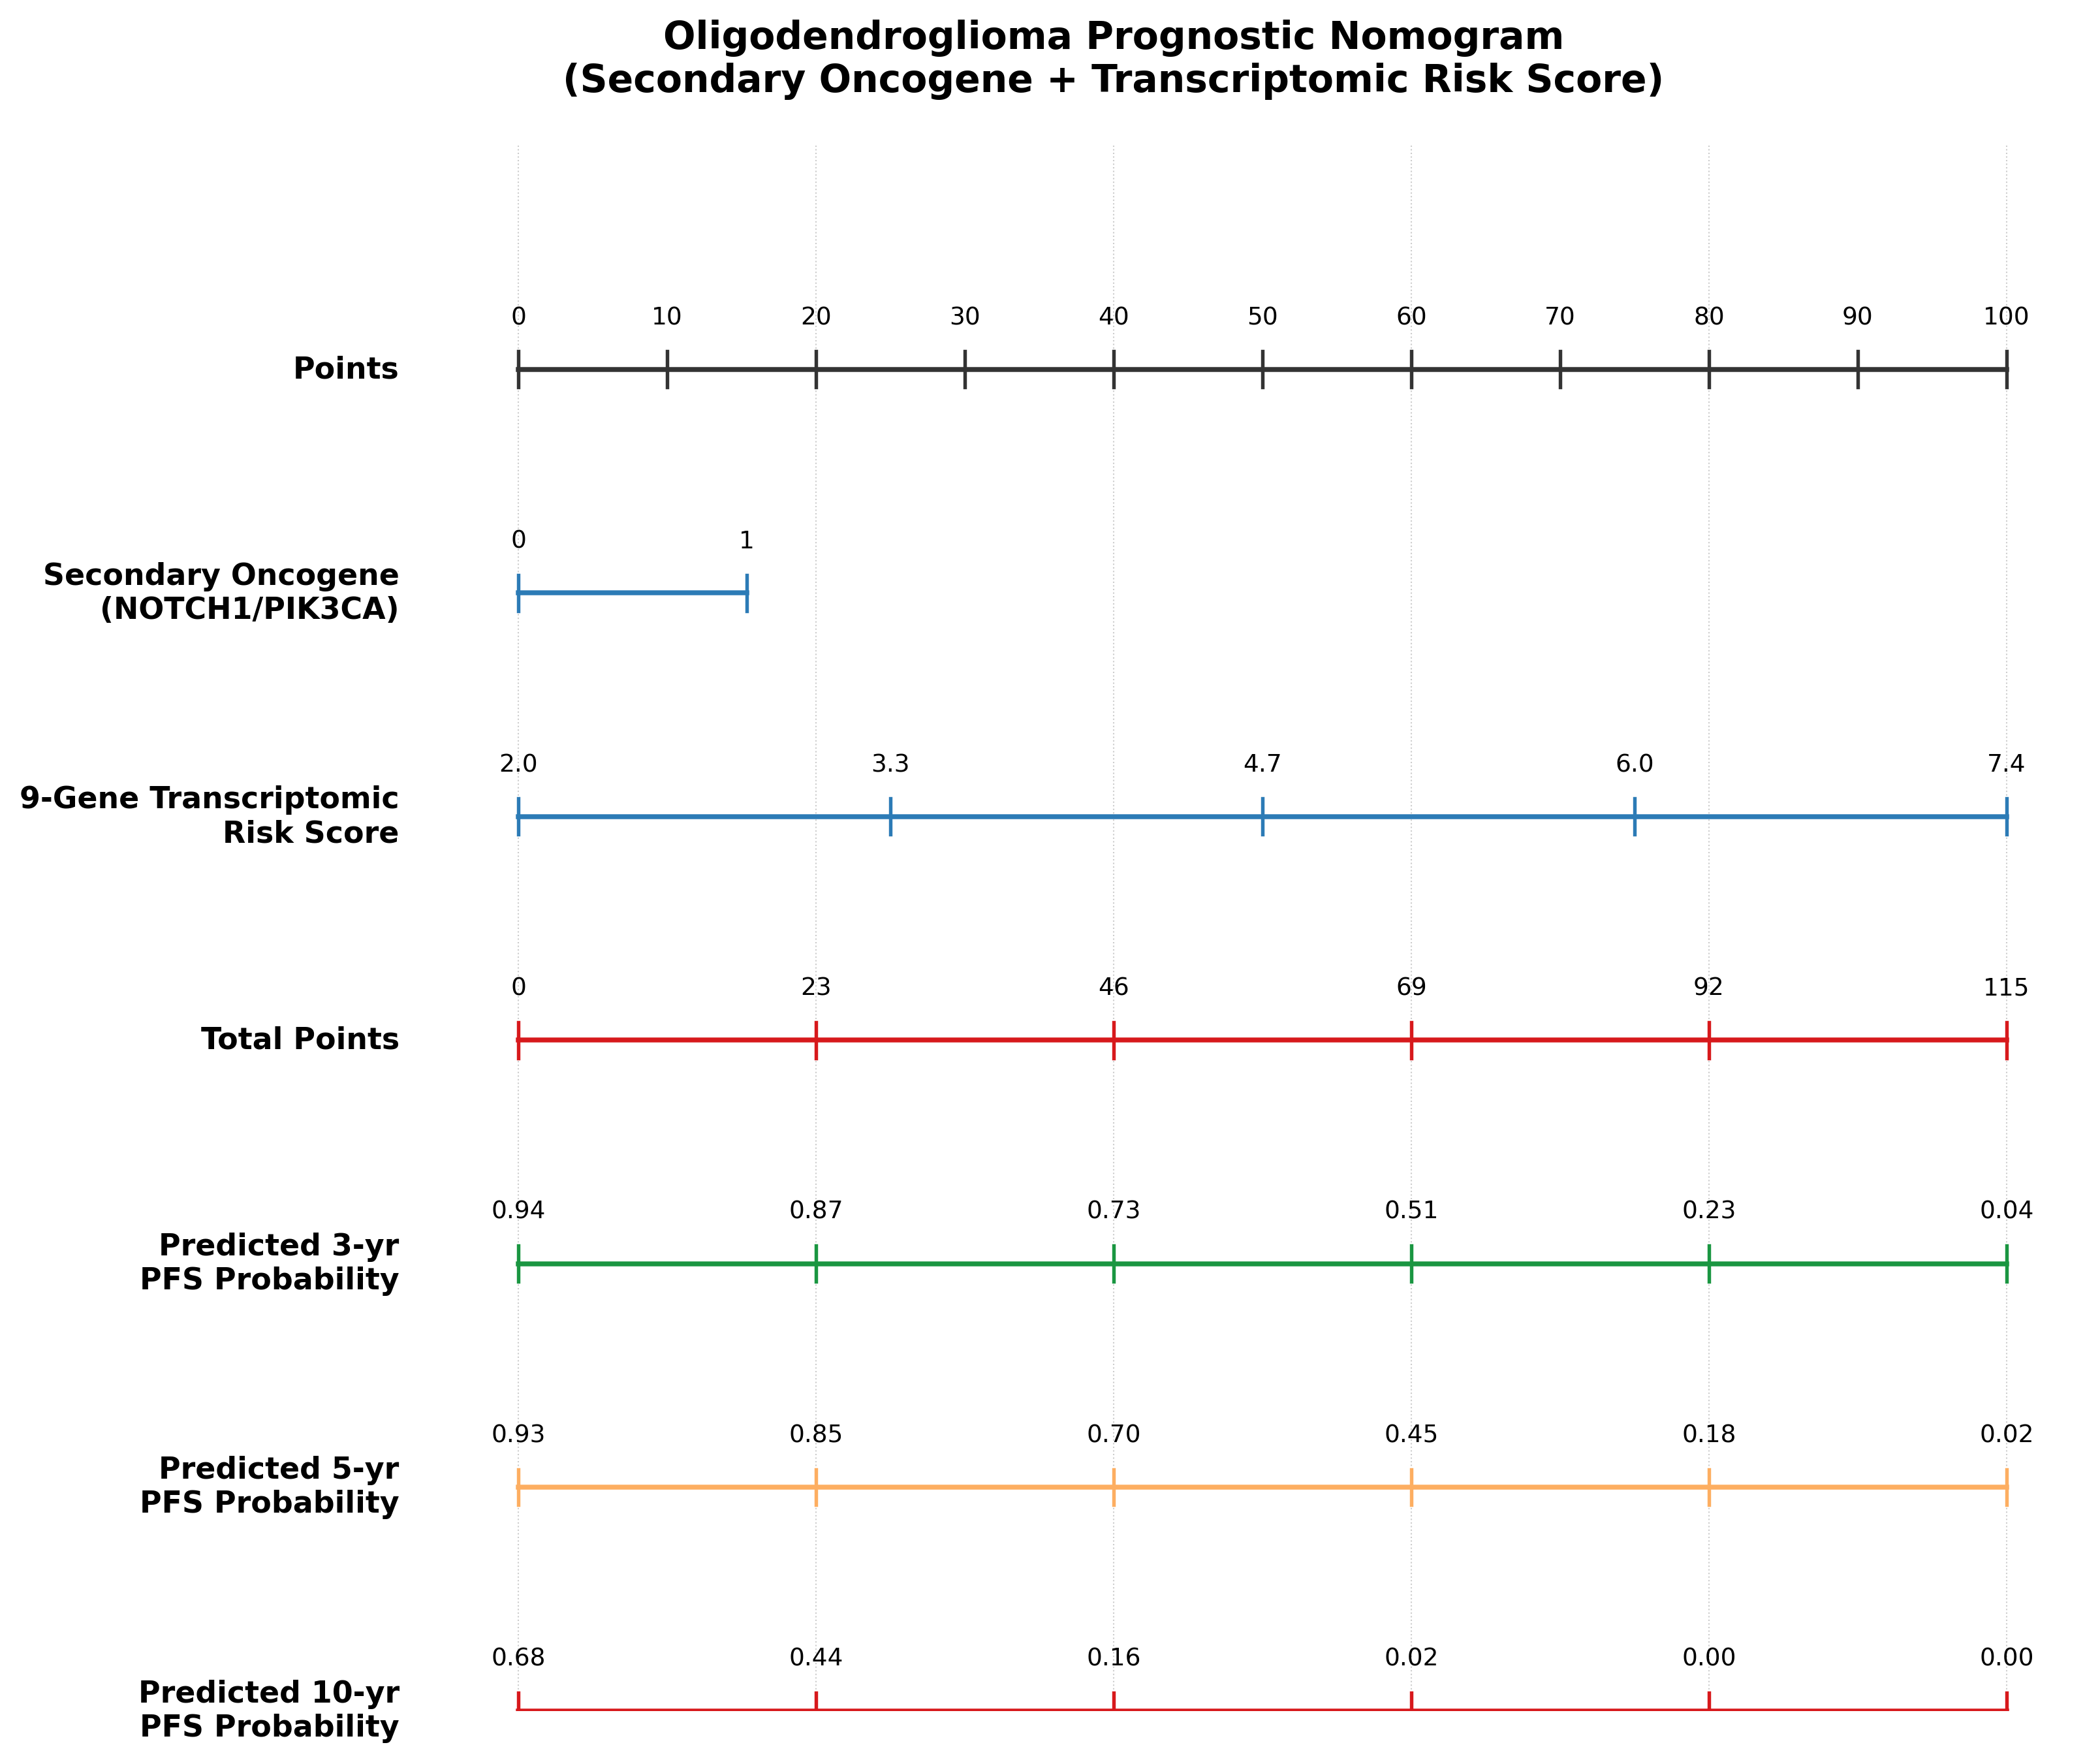
\includegraphics[width=0.75\linewidth]{16_nomogram.png}
    \caption{Two-variable prognostic nomogram.}
    \label{fig:nomogram}
\end{figure}

\subsection{Patient-Level Prediction Tool}

Two representative, synthetic patient profiles illustrate the prediction tool's output. A favorable profile (Grade II, age 32, no secondary oncogene, low-risk gene expression pattern) yielded a transcriptomic score at the 0.8th percentile of the training cohort, a LOW RISK classification. They were predicted 10-year progression-free survival probability of 77.2\%. An unfavorable profile (Grade III, age 58, secondary oncogene present, extremely high-risk gene expression pattern) yielded a score at the 100th percentile, a HIGH RISK classification, and a predicted 10-year progression-free survival probability of 0.0\% (and 1-year probability of 32.6\%) (Table~\ref{tab:predictions}), illustrating the spread in predicted outcomes the model produces across observed patient profiles.

\begin{table}[h!]
\centering
\caption{Predicted progression-free survival probability, representative patient profiles}
\label{tab:predictions}
\begin{tabular}{lcccc}
\toprule
Profile & Risk Class & 1-yr PFS & 5-yr PFS & 10-yr PFS \\
\midrule
Favorable (Grade II, age 32, no 2\textdegree\ oncogene) & LOW & 99.2\% & 95.1\% & 77.2\% \\
Unfavorable (Grade III, age 58, 2\textdegree\ oncogene present) & HIGH & 32.6\% & 0.1\% & 0.0\% \\
\bottomrule
\end{tabular}
\end{table}

The model was further updated to directly calculate patient transcriptomic risk score through the input of a TCGA-formatted mRNA-seq csv file for easier use, rather than requiring users to calculate the transcriptomic risk score manually.

\section{Discussion}

This project combined mutation, transcriptomic, and epigenetic data into a single, internationally validated risk model for oligodendroglioma, a tumor type whose current survival variation is underdeveloped and under-researched. Several key findings are worth discussing to provide context and reasoning as to why the results were achieved.

The secondary oncogene finding (NOTCH1/PIK3CA) is almost a validation of the model, and more of a confirmatory result of prior research literature. NOTCH1 mutations have previously been shown to predict worse survival in oligodendroglioma \cite{Aoki2018}, and computational work has also suggested that the PI3K pathway is important \cite{CancerGenomeAtlas2015}. The contribution of this study regarding secondary-oncogene impact is more methodological rather than discovery-based. The association was confirmed inside a cohort where histologically misclassified cases (32\% of the initial TCGA sample) had already been removed, which is a step prior studies might have missed. 

The specific nine-gene combination as a whole do not appear in literature. Neither does this specific application of LASSO-cox to oligodendroglioma appear, aside from the POLA network's own, differently-composed eight-gene signature \cite{Bertucci2023}. The Gene Set Enrichment Analysis helps to provide biological understanding and reasoning as to why the genes are of importance. For example, the most enriched pathways were centered on the cell cycle and proliferation, which is consistent with established cancer biology rather than an arbitrary statistical artifact of the LASSO methodology.

The PAX5 methylation finding also raises a question. Promoter methylation typically silences gene expression, so the positive correlation observed between PAX5 methylation and PAX5 expression (r= 0.570) runs against that expectation. Possible explanations include methylation occurring at CpG sites outisde of the core silencing region (which the project filtered out), an unmeasured phenomenon such as a tumor cell composition driving both measurements upward causing synthetic correlation, or a previously unreported relationship specific to this gene in oligodendroglioma. All of these ideas have some sort of validity, but this project cannot give a definitive answer. Furthermore, the inclusion of MGMT as a reference gene in the methylation screen, and its expected null result within this specific molecular subgroup, supports that the promoter-probe mapping and filtering pipeline was functioning correctly rather than arbitrarily producing PAX5's result. However, it still may be possible (though unlikely) that the correlation came from lack-of-data of PAX5 methylation specifically.

There is also a consistent pattern in both the secondary oncogene and PAX5 methylation results. They both independently add significance on their own, but they both lost significance once the transcriptomic score was added to the same model. This suggests that these three layers are not fully independent, and that some of the secondary oncogene status and PAX5 methylation capture is also being overlapped by the transcriptomic score. This is a caveat to the "multi-variable" framing of this model: the layers appear correlated rather than independently additive. This may also be because of lack-of-data again, although with bootstrap correction, schoenfeld residual tests, and repeated cross validation it seems unlikely.

Regarding CGGA validation results, the together illustrate an important understanding as to what has been confirmed externally and what has not. The transcriptomic score validated successfully as a direct, unmodified transfer to an independent population with a verified log-rank p score.  The clinical variables showed reasonable cross-cohort consistency, primarily showing the validity of the methodology. The individual, major biological signatures, by contrast, could not be confirmed in CGGA. This was most likely due to insufficient statistical power rather than absence of effect, given the extremely large confidence intervals observed. Because the clinical cohort (n=182) and the transcriptomic validation cohort (n=171) are not identical patient sets, it is also important to note that the full combined model has not been validated as a whole in CGGA due to the lack of a unanimous dataset with all the data required. Only the individual components have each been checked separately within different subsets of the broader CGGA population.

\subsection{Limitations}

A few limitations need to be emphasized and considered. First, the full model was fit on 125 patients with 35 events across covariates, below common statistical rules of thumb. The bootstrap-corrected concordance (0.82 vs 0.84) shows this, and true generalization of the model may even be slightly lower. Second, external validation currently only covers transcriptomic score and clinical layer, but both separately. The full model has not yet been validated as a whole (only by layers). However, work is currently being done to externally validate the model as a whole, including methylation data as well as all the other variables through a planned third cohort. Third, methylation platform differences across cohorts may limit the usage of the PAX5 finding specifically for methylation, since promoter probe coverage is not necessarily identical across differing dataset array versions. Fourth, the individual mutation-based major biological signature marker validation in CGGA was likely underpowered, due to there being even fewer events/deaths, limiting what can be concluded from its null result. 

\subsection{Future Directions}

Future work includes completing external validation of the full combined model using clinical and molecular data from the third international network, investigating the validity and mechanical aspects of the PAX5 methylation-expression relationship, and refining the transcriptomic signature as additional independent cohorts.

\section{Conclusion}

By restricting analysis to a strictly molecularly confirmed cohort, this study confirmed a known prognostic role for secondary oncogene mutations, identified PAX5 promoter methylation as a novel and independently significant, although mechanistically unresolved, prognostic marker, and combined these with a novel nine-gene transcriptomic risk score, supported by pathway enrichment analysis, into a multi-layer model reaching a bootstrap-corrected concordance of 0.82. The transcriptomic score was independently validated in an external Chinese cohort, and the model was translated into both a simplified nomogram and a full patient-level prediction tool. External validation of the complete combined model in a third, international cohort is in the process.

\section*{Acknowledgments}

I thank my mentor, Elyse Onstott, at the National Center for Genome Resources, 
for introducing me to computational biology and helping me chase my goals.

The results here are based upon data generated by the TCGA Research Network: https://www.cancer.gov/tcga. I am grateful to the patients whose contributions made this data publicly available for research. I am also thankful for the CGGA network: https://www.cgga.org.cn/.

I thank my father, who inspired me to take action against the disease impairing his life.

% References
\begin{thebibliography}{99}

\bibitem{WHO2021}
Louis DN, Perry A, Wesseling P, et al.
The 2021 WHO Classification of Tumors of the Central Nervous System: a summary.
\textit{Neuro-Oncology}. 2021;23(8):1231--1251. doi:10.1093/neuonc/noab106

\bibitem{CancerGenomeAtlas2015}
Cancer Genome Atlas Research Network.
Comprehensive, Integrative Genomic Analysis of Diffuse Lower-Grade Gliomas.
\textit{New England Journal of Medicine}. 2015;372(26):2481--2498. doi:10.1056/NEJMoa1402121

\bibitem{Aoki2018}
Aoki, K., Nakamura, H., Suzuki, H., et al.
Prognostic Relevance of Genetic Alterations in Diffuse Lower-grade Gliomas.
\textit{Neuro-Oncology}. 2018;20(1):66--77. doi:10.1093/neuonc/nox132

\bibitem{Bertucci2023}
Bertucci, A., et al.
A Multigene Signature Associated with Progression-Free Survival after Treatment for IDH Mutant and 1p/19q Codeleted Oligodendrogliomas.
\textit{Cancers}. 2023;15:3067. doi:10.3390/cancers15123067

\bibitem{Friedman2010}
Friedman J, Hastie T, Tibshirani R.
Regularization Paths for Generalized Linear Models via Coordinate Descent.
\textit{J Stat Softw}. 2010;33(1):1--22. doi:10.18637/jss.v033.i01

\bibitem{Cox1972}
Cox DR.
Regression Models and Life-Tables.
\textit{J R Stat Soc Series B}. 1972;34(2):187--220.

\bibitem{Goldman2020}
Goldman MJ, Craft B, Hastie M, Repečka K, McDade F, Kamath A, et al.
Visualizing and Interpreting Cancer Genomics Data via the Xena Platform.
\textit{Nature Biotechnology}. 2020;38(6):675--678.
doi:10.1038/s41587-020-0546-8

\bibitem{OncoKB2017}
Chakravarty D, Gao J, Phillips SM, et al.
OncoKB: A Precision Oncology Knowledge Base.
\textit{JCO Precision Oncology}. 2017;1:1--16. doi:10.1200/PO.17.00011

\bibitem{Subramanian2005}
Subramanian A, Tamayo P, Mootha VK, et al.
Gene Set Enrichment Analysis: A Knowledge-Based Approach for Interpreting Genome-Wide Expression Profiles.
\textit{Proc Natl Acad Sci USA}. 2005;102(43):15545--15550. doi:10.1073/pnas.0506580102

\bibitem{Hegi2005}
Hegi, M. E., Diserens, A. C., Gorlia, T., et al.
MGMT Gene Silencing and Benefit from Temozolomide in Glioblastoma.
\textit{New England Journal of Medicine}. 2005;352:997--1003. doi:10.1056/NEJMoa043331

\bibitem{Hallmark2015}
Liberzon A, Birger C, Thorvaldsdóttir H, et al.
The Molecular Signatures Database Hallmark Gene Set Collection.
\textit{Cell Syst}. 2015;1(6):417--425. doi:10.1016/j.cels.2015.12.004

\bibitem{Bibikova2011}
Bibikova M, Barnes B, Tsan C, et al.
High density DNA methylation array with single CpG site resolution.
Genomics. 2011;98(4):288--295. doi:10.1016/j.ygeno.2011.07.007

\bibitem{Zhao2021}
Zhao Z, Zhang KN, Wang Q, et al.
Chinese Glioma Genome Atlas (CGGA): A Comprehensive Resource with Functional Genomic Data from Chinese Glioma Patients. Genomics, Proteomics & Bioinformatics. 2021.

\end{thebibliography}


\end{document}
